\documentclass{article}
  \parindent = 0mm % Sin sangría
  \usepackage[utf8]{inputenc}
  \usepackage[T1]{fontenc}
  \usepackage[spanish]{babel}
  \usepackage{graphicx}
  \usepackage{amstext}
  \usepackage{amsmath}
  \usepackage{amsthm}
  \usepackage{booktabs}
  \usepackage{subfigure}
  \usepackage{footnote}
  \usepackage{hyperref}
  \usepackage{algpseudocode,algorithm,algorithmicx}
  \usepackage[font=small,labelfont=bf]{caption}
  \usepackage{esvect}

  \newtheorem{definition}{Definición}
  \newtheorem{lemma}{Lema}

  \newcommand{\modelspace}{\hspace{1.5em}}

\begin{document}
  \begin{center}
    {\sc \large Maestría en Investigación de Operaciones}

    {\sc \large Tesis - Borrador}
    \linebreak

    {\rm Joaquín Correa - \today}
  \end{center}

  \section*{Introducción}

  Es de sorprendente espectro los beneficios obtenidos por utilizar la bicicleta como medio de transporte. No siempre es posible hacerlo debido a factores como la distancia del viaje, situaciónes climáticas adversas como lluvias, frio o calor, falta de infrastructura vial entre otras. La bicicleta es una alternativa particularmente favorable en viajes cortos en comparación al uso de automóvil o transporte colectivo (TODO: referencia del paper 2021 lim). En Uruguay una proporción signifitiva de la población sufre factores de riesgos cardiovasculares como sedentarismo, obesidad o hipertension (\ref{heartrisksuy}) que pueden ser prevenidos en cierta medida con ejercicio frecuente moderado como es el transporte en bicicleta (\ref{mspphisicalactivityguid}) (\ref{mspsurveyriskfactors}). La sustitución de transporte privado automotor por bicicleta tambien es favorable en el descongestionamiento de calles y consiguiente dismunusión en la contaminación del aire y sonora, problemas que son comunes en ciudades grandes. En este trabajo se propone un método exacto para el problema de la atracción de demanda desde un modo (o un agregado de modos) de transporte a la bicicleta. Se discuten algunas consideraciones de la formulación para ser llevada a un problema lineal y se analizan los parámetros mas relevantes. Finalmente se aplica el problema a la ciudad de Montevideo.

  \section*{Problema}

  \subsection*{Descripción}

  El problema se ubica dentro del contexto de diseño y planificación de ciclovías en una ciudad.

  Dada una red que modela una ciudad y una matriz origen-destino con demanda asociada, el objetivo es maximizar la cantidad de demanda que utiliza la bicicleta como modo de transporte. Para poder lograr esto, se cuenta con infraestructuras y presupuesto, que de ser utilizados, permiten disminuir el costo percibido por el usuario al utilizar la bicicleta, asumiendo que utiliza el camino más corto, y por lo tanto potencialmente influir la decisión de utilizarla como modo de transporte.

  \subsection*{Formulación}

  En este trabajo se parte de una formulación binivel del problema dado que es una representación directa de lo que se quiere resolver. El primer nivel representa la comuna (o entidad que toma decisiónes sobre las ciclovías) y maximiza la cantidad de usuarios que utilizan la bicicleta por medio de la decisión de la ubicación y tipo de ciclovías para cada arco de la red. El segundo nivel representa a los usuarios y resuelve el problema del costo del camino más corto para cada par de nodos origen-destino. En principio los objetivos de los subproblemas no son directamente agregables ni es posible solucionar este problema tal cual está con un solver por lo que se estudiarán maneras de reformularlo y formulaciones alternativas.

  Las hipótesis que se asumieron para este trabajo son:

  \begin{itemize}
    \item{El tiempo de viaje en todo arco de la red es independiente del flujo sobre el mismo.}
    \item{Existen diferentes pares origen-destino de demanda en la red y para cada par origen-destino existen diferentes caminos que unen el origen y el destino.}
    \item{Los usuarios siempre buscan minimizar el costo de su viaje (todos son
    perfectos optimizadores y se comportan igual)}
  \end{itemize}

  Sobre la red, consideramos que los grafos son dirigidos y cuando se decide construir una infraestructura sobre un arco solo se hace en la dirección del arco. Esto simplifica el modelado pero puede no ser tan realista considerando que el costo marginal de construir una infraestructura dado que existe la misma infraestructura en el otro sentido es menor al costo de construir la primera. Tambien puede resultar en que dado dos nodos adyacentes mutuamente, se decida construir diferentes infraestructuras en cada sentido. Sin embargo, dado que en general las redes que modelan las ciudades sobre las que se quieren resolver estos problemas son una simplificación de la red de calles, las consideraciones irreales mencionadas no tienen consecuencia práctica.

  Puede observarse que la formulación propuesta considera aspectos de modelos descriptivos, en donde el objetivo es simular el comportamiento de los usuarios, y modelos normativos (o de optimización) en donde el objetivo es mejorar las decisiones que afectan un proceso. TODO: Referencias y mencion sobre complejidad de mezclar ambos.

  \subsection*{Formulación matemática}

  Sean los siguientes conjuntos y parámetros:

  \begin{description}
    \item[$OD$]: Conjunto de pares origen destino con elemento genérico $k$.
    \item[$G=(N,A)$]: Grafo dirigido que modela la red, con su conjunto de nodos $N$ y de arcos $A$. $A_n^+$ y $A_n^-$ son los conjuntos de arcos que salen y entran respectivamente desde el nodo $n$.
    \item[$I$]: Conjunto de infraestructuras de ciclovías.
    \item[$C_{ai}$]: Costo de usuario de atravesar el arco $a \in A$ utilizando la infraestructura $i \in I$. $C_{ai} > 0$.
    \item[$H_{ai}$]: Costo de construcción de la infraestructura $i \in I$ en el arco $a \in A$. $H_{ai} \geq 0$ .
    \item[$B$]: Presupuesto para la construcción de infraestructuras.
    \item[$\theta_{nk}$]: Parámetro que vale 1 si n es el origen del par origen-destino $k \in OD$, -1 si es el destino y 0 en otro caso.
    \item[$w_k$]: Variable de primer nivel que contiene el valor del camino más corto para el par origen destino $k \in OD$.
    \item[$y_{ai}$]: Variable binaria de primer nivel que determina si la infraestructura $i \in I$ está activa en el arco $a \in A$.
    \item[$x_{ak}$]: Variable de segundo nivel que determina si el arco $a \in A$ es parte del camino más corto para el par origen-destino $k \in OD$.
    \item[$f_k$]: Función que determina la demanda que utiliza la bicicleta como modo de transporte en función del costo del camino mas corto.
  \end{description}

  \begin{align}
    \text{max}    & \sum_{k \in OD} f_k(w_k)                                                         & \label{eq:objective1lvl} \\
    \text{s.t.}\; & w_k = \sum_{a \in A} \sum_{k \in OD} \sum_{i \in I} C_{ai}y_{ai}x_{ak}           & \forall k \in OD \label{eq:shortestpath} \\
                  & B \geq \sum_{a \in A} \sum_{i \in I} H_{ai}y_{ai}                                & \label{eq:respectbudget} \\
                  & 1 = \sum_{i \in I} y_{ai}                                                        & \forall a \in A \label{eq:alwaysoney} \\
                  & w_k \geq 0, y_{ai} \in \{0,1\}                                                   & \nonumber \\
                  & \text{min} \sum_{a \in A} \sum_{k \in OD} \sum_{i \in I} C_{ai}y_{ai}x_{ak}      & \label{eq:subproblem} \\
                  & \text{s.t.} \sum_{a \in A_n^+} x_{ak} - \sum_{a \in A_n^-} x_{ak} = \theta_{nk}  & \forall n \in N, k \in OD \label {eq:flowbalance} \\
                  & \modelspace x_{ak} \geq 0                                                        & \nonumber
  \end{align}

  Donde:

  \begin{description}
    \item[\ref{eq:objective1lvl}]: La función objetivo es la suma de los valores de demandas que cambiaron de modo de transporte.
    \item[\ref{eq:shortestpath}]: Restricción que determina el costo del camino más corto dado en el primer nivel.
    \item[\ref{eq:respectbudget}]: Restricción de presupuesto sobre lo que se puede construir.
    \item[\ref{eq:alwaysoney}]: Restricción que requiere que una infraestructura estar activa en cada arco. Se discutirá más sobre esto en la siguiente sección.
    \item[\ref{eq:subproblem}]: Función objetivo del segundo nivel.
    \item[\ref{eq:flowbalance}]: Restricción de balance de flujo.
  \end{description}

  \subsubsection*{Observaciones}

  La linealidad de la formulación propuesta es determinada por las funciónes $f_k$. En las ecuaciones (\ref{eq:shortestpath}) y (\ref{eq:subproblem}) las variables de primer y segundo nivel se multiplican pero dado que las variables de un nivel son parámetro en el otro nivel no se pierde la linealidad de dichas ecuaciónes.

  En la formulación del problema de primer nivel, la restricción (\ref{eq:alwaysoney}) pudo haber sido escrita de manera que al menos una infraestructura esté activa. Esto se puede ver de diferentes maneras, pensando en la realidad modelada, un ciclista podría pasar prácticamente por cualquier calle sin problemas, entonces para que las instancias del modelo sean semánticamente correctas debería existir una infraestructura $i_0 \in I$ cuyo costo de construcción $H_{ai_0}$ sea 0 en todos de los arcos $a \in A$, mas allá de que el costo de usuario pueda ser altísimo. Desde un punto de vista formal, como se verá mas adelante, si no se requiere que en cada arco haya una infraestructura activa, entonces hay que agregar al problema de segundo nivel una restricción que evite que se activen flujos en arcos donde no hay infraestructura activa, es decir: $x_{ak} \leq \sum_{i \in I} y_{ai}, \forall a \in A, k \in OD$. Con esta restricción, el problema de segundo nivel puede no tener solución factible cuando las infraestructuras seleccionadas por el primer nivel no inducen un subgrafo que conectan todos los pares origen-destino.

  Se asumirá de aquí en adelante que las instancias del problema están bien definidas, esto significa que:

  \begin{enumerate}
    \item {$G$ es conexo}
    \item {$\forall k \in OD$ existe un camino $S_k \in G$ con costo de construcción cero, es decir $\sum_{a \in S_k} H_{ai_0} = 0$}
  \end{enumerate}

  \section*{Consideraciones semánticamas}

  Es de particular interés para la formulación los parámetros que representan la demanda y funciones de transferencia de demanda entre modos. Se incurre en una simplificación que reduce todos los modos existentes, por ejemplo transporte público, taxi o privado; a uno y considera la transferencia desde este modo agregado a la bicicleta. Luego, en función del dominio de las funciones de transferencia es que debe especificarse los valores de demanda entre pares origen-destino.

  \subsection*{Validación de la formulación}

  Para discutir la validez del modelado se utilizará una formulación estándar de problema binivel o BLPP (Bi Level Programming Problem), como se puede encontrara en Bard (\ref{bardbook}).
  Sea la siguiente formulación simplificada del problema:

  \begin{align}
    \text{max}_{y \in Y}    & \; F(x, y) \\
    \text{s.t.} \modelspace & A_1 x + B_1 y \leq b_1 \\
                            & \text{min}_{x \in X} f(x, y) \\
                            & \modelspace A_2 x + B_2 y \leq b_2
  \end{align}

  Y las siguientes definiciones:

  \begin{definition}
    Conjunto factible
    \begin{align}
      S = \{(x, y) \setminus x \in X, y \in Y, A_1 x + B_1 y \leq b_1, A_2 x + B_2 y \leq b_2 \}
    \end{align}
  \end{definition}

  \begin{definition}
    Conjunto de reacción del segundo nivel:
    \begin{align}
      P(y) = \{ x \in \text{argmin}_{\hat{x} \in X} f(\hat{x}, y) : A_2 \hat{x} + B_2 y \leq b_2 \}
    \end{align}
  \end{definition}

  Diremos que el problema está bien formulado si el conjunto $S$ es no vacío, es decir, si existen soluciones factibles y si para toda $y$ el conjunto $P(y)$ es no vacío, es decir, si para todo movimiento del problema de primer nivel, hay margen de decisión en el segundo nivel.

  \begin{lemma}$S$ es no vacío
  \end{lemma}

  \begin{proof}
    $S \neq \emptyset$ ya que $\exists (x_0, y_0) \in X \times Y$ donde $y_0$ es el vector $y_{ai_0} = 1 \forall a \in A$, $i_0$ es la infraestructura cuyo costo $H_{ai_0} = 0$, lo que deja al resto de las entradas del vector $y_0$ en $0$. Por lo tanto se cumple las restricción (\ref{eq:alwaysoney}) dado que todos los arcos tienen una infraestructura activa, y la restricción (\ref{eq:respectbudget}) dado que el costo total de construcción de $y_0$ es $0$.

    Luego, dado que las infraestructuras activas logran la conectividad de los pares origen-destino y el hecho de que el el costo de los arcos $C_ai$ sea no negativo permite asegurar que el problema de segundo nivel tiene al menos una solución factible $x_0$.
  \end{proof}

  \begin{lemma}$\forall y \in Y,\; P(y) \neq \emptyset$
  \end{lemma}

  \begin{proof}
    Para cualquier asignación $y = \hat{y} \in Y$, se cumple que $P(\hat{y})$ es no vacío ya que todos los arcos tienen una infraestructura activa, por lo tanto el grafo donde los flujos del problema de segundo nivel pueden pasar es conexo y llega necesariamente a todos los nodos, incluyendo los pares origen-destino. Por lo tanto el espacio de soluciones factibles del subproblema es no vacío. 
  \end{proof}

  Aún cuando estas dos definiciones se cumplen, puede haber dificultades al encontrar la solución óptima cuando $P(y)$ contiene más de un elemento, caso en el cual el modelo puede no llegar a la solución óptima, dependiendo del valor $x \in P(y)$ que seleccione el problema de segundo nivel. En este caso de estudio esto es muy probable que suceda, puesto que pueden haber varios caminos más cortos entre dos puntos.

  \section*{Resolución del problema BLPP}

  Si bien la formulación binivel expresa de buena manera lo que se quiere resolver, en la práctica los BLPP son en general de dificil resolución, ya se ha demostrado en Bard (\ref{bardbook}) que el BLPP lineal es NP-Hard. Por eso se analizará una formulación alternativa como LP de un nivel.

  \subsection*{Transformación de binivel a un nivel}

  Este problema se puede transformar a un problema de un nivel sustituyendo el problema de segundo nivel por sus restricciónes de optimalidad de KKT en el primer nivel. De obtenerse una representación lineal se podría buscar alguna metodología exacta para resolverlo. La formulación binivel estudiada presenta el problema, a los efectos de la transformación, de contener ecuaciones con variables de diferentes niveles multiplicándose, dichas ecuaciones deben ser reformuladas para que no devengan en restricciones no lineales.

  \subsection*{Formulación alternativa de un nivel}
  \label{altOneLevelFormulation}

  A diferencia de la transformación a un nivel que podemos decir que genera una formulación equivalente a la binivel, en esta sección se propone una formulación alternativa que se entiende equivalente. Equivalente en qué sentido? Esto depende de lo que se quiere obtener de la resolución del problema. Podemos decir que al menos debe ser equivalente en terminos del objetivo, es decir, cantidad de demanda transferida, ademas puede interesar (e interesa) la decisión de dónde construir qué infraestructuras y flujos óptimos. Parece sensato afirmar que si la nueva formulación busca optimizar el mismo objetivo entonces las decisiones tomadas van a ser equivalentes, no necesariamente las mismas, pero dentro del conjunto de decisiones que el sujeto interpretante toma como válidas.

  Esta formulación nace de la formulación binivel quitando el subproblema y agregando sus restricciones al problema de primer nivel bajo el argumento de que las funciones $f_k$ deben ser decrecientes, entonces para maximizar $\sum_{j \in OD}f_k(w_k)$ lo mejor es los $w_k$ sean lo más chico posible.

  La formulación resultante es la siguiente:

  \begin{align}
    \text{max}    & \sum_{k \in OD} f_k(w_k)                                                         & \label{eq:objectivealt} \\
    \text{s.t.}\; & w_k = \sum_{a \in A} \sum_{k \in OD} \sum_{i \in I} C_{ai}y_{ai}x_{ak}           & \forall k \in OD \label{eq:shortestpathalt} \\
                  & B \geq \sum_{a \in A} \sum_{i \in I} H_{ai}y_{ai}                                & \label{eq:respectbudgetalt} \\
                  & 1 = \sum_{i \in I} y_{ai}                                                        & \forall a \in A \label{eq:alwaysoneyalt} \\
                  & \sum_{a \in A_n^+} x_{ak} - \sum_{a \in A_n^-} x_{ak} = \theta_{nk}              & \forall n \in N, k \in OD \label{eq:flowbalancealt} \\
                  & w_k \geq 0, x_{ak} \geq 0, y_{ai} \in \{0,1\}                                    & \nonumber
  \end{align}

  \subsubsection*{Observaciones}

  Puede considerarse que la formulación corresponde a la optimización de Pareto de ambos problemas de la formulación binevel considerando factores 1 para el primer nivel y 0 para el objetivo del segundo nivel. Queda por analizar el efecto de quitar el objetivo del segundo problema de la función objetivo y si, en todo caso, la optimización de Pareto resuelve lo buscado.

  \subsection*{Quitando multiplicación de variables}

  El objetivo es quitar la multiplicación entre $x_{ak}$ e $y_{ai}$. Se propone la formulación siguiente del problema de segundo nivel.

  \begin{align}
    \text{min}  & \sum_{k \in K} \sum_{a \in A} \sum_{i \in I} C_{ai} h_{aki}         & \label{eq:subproblemrefeq1} \\
    \text{s.t.} & \sum_{a \in A_n^+} x_{ak} - \sum_{a \in A_n^-} x_{ak} = \theta_{nk} & \forall n \in N, k \in OD \\
                & 0 \leq h_{aki} \leq y_{ai}                                          & \forall a \in A, k \in K, i \in I \\
                & x_{ak} = \sum_{i \in I} h_{aki}                                     & \forall a \in A, k \in K
  \end{align}

  Si utilizamos la ecuación (\ref{eq:subproblemrefeq1}) en la restricción de igualdad de $w_k$ (ecuación \ref{eq:shortestpath}) el problema es equivalente con la ventaja que no existen variables de diferentes niveles multiplicándose. La equivalencia se da porque esta formulación desagrega los flujos para cada infraestructura ademas de par origen-destino y arco en la variable $h_{aki}$, que es lo que se modela con con $y_{ai} x_{ak}$.

  \subsection*{Definición de las $f_k$s}

  Estas funciones fueron dejadas de lado en la formulación inicial con el objetivo de analizar las restricciones principales primero. Se analizan en esta sección diferentes alternativas de cómo implementarlas como un conjunto de ecuaciones lineales que se acoplaran a las formulación antedicha.

  Podemos encontrar en la literatura soluciones a problemas similares. En Laporte 2007 (\ref{laporte2007}) y Lim 2021 (\ref{lim2021}), donde se considera un parámetro $c^{PRIV}_k$ que modela el costo del transporte privado para un par origen-destino $k$, si la red de transporte público logra un costo menor entonces se considera que toda la demanda del par origen-destino $k$ se transfiere a dicho modo.

  \subsubsection*{Definición propuesta}

  Se considera que una función $f_k$ arbitraria debe poder modelar una transición paulatina de la demanda entre modos de transporte. Paulatina de manera de expresar una transición que pueda parecerse a algo lineal, exponencial o lo que fuere. Asumiendo que las $f_k$ son decrecientes, la mejor forma que ocurriese es representarla como una sucesión decreciente de puntos de quiebre, tal que para cada uno se exista un valor asociado de cantidad de demanda transferida. Los puntos de quiebre son comparados contra el valor del camino más corto $w_k$. Entonces sea $w_k$ fijo, la demanda transferida es:

  \begin{equation}
    \label{eq:deffks}
    f_k(w_k) = P_{j^*},\; j^* = argmin_{j \in J} \{Q_j \geq w_k\}
  \end{equation}
  
  Donde $Q_j$ son los puntos de quiebre en la unidad del costo del camino más corto, $J$ es un conjunto índice y $P_{j^*}$ es la cantidad de demanda que se transfiere. Una ventaja de esta formulación es que puede ser integrada a la función objetivo de la formulación inicial de manera que la minimización queda en manos del objetivo del mismo problema.

  Como alternativa, se puede podría pensar una definición de $f_k$ como función no lineal, esto puede llevar a soluciones soluciones analíticamente más precisas pero es sabido que aumenta considerablemente la dificultad de resolución práctica.

  Para modelar la función $argmin$ en una formulación como la que se viene trabajando es necesario utilizar variables de activación que solo permita que una entrada del índice esté activo. Por ejemplo si se usa $z_j,\; j \in J$, lo antedicho equivale a decir que $z_j \in \{0,1\}$ y $\sum_{j \in J} z_j = 1$. Como estas restricciones se encuentran dentro de una maximización y suponiendo que el conjunto ordenado $Q$ es estrictamente decrecientes, podemos relajar la restricción de integralidad y sustituirla por $0 \leq z_j \leq 1$. Es esperable pensar que no pueden existir varios $z_j$ activos para la definición (\ref{eq:deffks}), porque si los hubiesen, al ser $Q$ y $P$ conjuntos ordenados estrictamente decreciente entonces no se llegaría al máximo.

  Nótese que esta definición es una extensión de la propuesta por Laporte 2007 (\ref{laporte2007}) y Lim 2021 (\ref{lim2021}). Para modelarla basta considerar $J = \{0, 1\}$, $P_0 = 0, P_1 = D_k$ y $Q_0 = M, Q_1 = c^{PRIV}_k$, donde $M$ es un numero arbitrario mayor a $c^{PRIV}_k$ y $D_k$ es la demanda para el par origen-destino $k$.

  \subsubsection*{Formulación de $f_k$ como LP}

  En esta sección se discuten diferentes formulaciones de $f_k$ como LP con el objetivo de analizar cómo se integrará a la formulación del problema que se quiere resolver. La forma más simple de modelar $f_k$ (ó simplemente $f$) es la (\ref{eq:fkv1eq1})-(\ref{eq:fkv1eq4}).

  \begin{align}
    f(W) =\; & max \sum_{j \in J} P_j y_j    & \label{eq:fkv1eq1}\\
             & s.t. \sum_{j \in J} y_j = 1   & \label{eq:fkv1eq2} \\
             & \;\;\; Q_j \geq W y_j         & \label{eq:fkv1eq3} \forall j \in J \\
             & \;\;\; y_j \in \{0,1\}        & \label{eq:fkv1eq4}
  \end{align}

  Si se intenta integrar esta formulación a (\ref{eq:objective1lvlfinal})-(\ref{eq:respectinfra}) el resultado seria un problema quadrático ya que $W$ sería sustituido por $w_k$. Por este motivo se estudiaron dos formulaciones alternativas que logran solucionar esta situación. La idea en ambas es desagregar $W$ como la suma de nuevas variables y utilizar estas en la restricción (\ref{eq:fkv1eq3}) en lugar de $W y_j$.

  \paragraph*{$f_k$ como LP version 1}

  \begin{align}
    f(W) =\; & max \sum_{j \in J} P_j y_j             & \label{eq:fkv3eq1}\\
             & s.t. \sum_{j \in J} y_j = 1            & \label{eq:fkv3eq2}\\
             & \;\;\; Q_j \geq w^{aux}_j              & \forall j \in J \label{eq:fkv3eq3} \\
             & \;\;\; w^{aux}_j \leq M y_j            & \forall j \in J \label{eq:fkv3eq4} \\
             & \;\;\; w^{sink}_j \leq M (1 - y_j)     & \forall j \in J \label{eq:fkv3eq5} \\
             & \;\;\; w^{sink}_j + w^{aux}_j = W      & \label{eq:fkv3eq6} \\
             & \;\;\; y_j \in \{0,1\}                 & \label{eq:fkv3domainy} \\
             & \;\;\; w^{aux}_j, w^{sink}_j \geq 0    & \label{eq:fkv3eq7}
  \end{align}

  Se desagrega $W$, para cada $j$ en $w^{sink}_j + w^{aux}_j$ de manera que uno de los dos tenga el valor de $W$, esto se logra con las restricciones (\ref{eq:fkv3eq4}) y (\ref{eq:fkv3eq5}). Entonces se cumple que solo el $w^{aux}_j$ cuyo $y_j$ esté activo tendrá el valor de $W$. Las mencionadas restricciones sirven para activar $y_i$ utilizado un parámetro $M \geq W$ arbitrario. Finalmente las restricciónes (\ref{eq:fkv3eq2}) y (\ref{eq:fkv3eq6}) logran que solo una de las variables $w^{aux}_j$ o $w^{sink}_j$ tome el valor de $W$, para cada $j$.

  \paragraph*{$f_k$ como LP version 2}

  \begin{align}
    f(W) =\; & max \sum_{j \in J} P_j y_j             & \label{eq:fkv2eq1}\\
             & s.t. \sum_{j \in J} y_j = 1            & \label{eq:fkv2eq2}\\
             & \;\;\; Q_j \geq w^{aux}_j              & \forall j \in J \label{eq:implfkoriginalineq} \\
             & \;\;\; w^{aux}_j \leq M y_j            & \forall j \in J \label{eq:yactivation1} \\
             & \;\;\; \sum_{j \in J} w^{aux}_j = W    & \label{eq:activatewaux} \\
             & \;\;\; y_j \in \{0,1\}                 & \label{eq:fkv2domainy} \\
             & \;\;\; w^{aux}_j \geq 0                & \label{eq:fkv2eq6}
  \end{align}

  En este caso se desagrega $W$ como suma de $|J|$ variables $w^{aux}_j$ de manera que solo una de ellas esté activa y tenga el valor de $W$. Para activar $y_i$ se agrega la restricción (\ref{eq:yactivation1}) utilizado, igual que en la formulación anterior, un parámetro $M \geq W$ y finalmente las restricciónes (\ref{eq:activatewaux}) y (\ref{eq:fkv2eq2}) logran que solo uno de los $w^{aux}_j$ tome el valor de $W$ y el resto sean 0.

  \subsubsection*{Validación de la formulación}

  Según definimos $f_k(W)$ en (\ref{eq:deffks}), sea de $p = f_k(W)$, entonces se cumple que:

  \begin{enumerate}
    \item {\label{deffpt1} $p$ es exactamente uno de los valores del conjunto de valores $P_j$, es decir: $p \in \{P_j\}_{j \in J}$}
    \item {\label{deffpt2} Sea $\hat{j} = j \;|\; p = P_j$. El valor del punto de quiebre $Q$ asociado a $\hat{j}$ no es menor que el costo del camino más corto $W$, es decir: $Q_{\hat{j}} \geq W$.}
    \item {\label{deffpt3} Dado el $\hat{j}$ anterior, entonces no existe un punto de quiebre $Q_j \forall j \in J$ que sea no mayor al punto de quiebre $Q_{\hat{j}}$ y mayor o igual al costo del camino más corto, es decir: $\not{\exists}\; Q_j\; \forall j \in J \;|\; Q_j \in  [W, Q_{\hat{j}}]$}.
  \end{enumerate}

  Es de interés analizar la correctitud de las formulaciones respecto a los puntos mencionados. En particular, la versión 2 (\ref{eq:fkv2eq1}) - (\ref{eq:fkv2eq6}) que es la que se utilizará finalmente. Se tiene que el punto \ref{deffpt1} se cumple, en la formulación, en la función objetivo (\ref{eq:fkv2eq1}) donde el valor objetivo es la suma de un subconjunto de $\{P_j\}_{j \in J}$, la restricción (\ref{eq:fkv2eq2}) que dice que solo uno de esos valores puede estar activo en la suma del objetivo y la restricción (\ref{eq:fkv2domainy}) que determina el carácter de la variable de decisión. El punto \ref{deffpt2} se cumple en la restricción (\ref{eq:implfkoriginalineq}), dado que $w^{aux}_j$ es igual a $W$ o cero, como se detalla en las restricciones (\ref{eq:yactivation1}), (\ref{eq:activatewaux}) y el carácter binario de $y_j$. Si $w^{aux}_j = W$, entonces el $j$ activo es el valor funcional de $f(W)$ y se cumple la definición del punto \ref{deffpt2}. Por otro lado, si es cero entonces el $j$ activo no es $\hat{j}$ y por lo tanto también se cumple el punto en cuestión. Finalmente, el punto \ref{deffpt3} se cumple por el hecho de que la función objetivo es una maximización y que $f(W)$ es una función estrictamente decreciente, entonces si existiera un $Q_a \in \{Q_j\}_{j \in J} \;|\; Q_a < Q_{\hat{j}}, a \in J$ entonces por se $f$ decreciente existe un valor $P_a > P_{\hat{j}}$ lo que contradice el hecho mismo de que el objetivo sea una maximización.

  \subsubsection*{Valores posibles de $P_j$ y $Q_j$}

  Para un $k \in OD$, sea $\overline{W}$ el costo del camino más corto sobre el grafo base (sin infraestructuras) y $\underline{W}$ el mejor costo del camino más corto suponiendo que las mejores infraestructuras se pueden construir, entonces $Q_j \in [\underline{W}, \overline{W}],\; \forall j \in J$\footnote{En realidad, $\overline{W}$ es el mínimo valor para el que $f_k$ es mínimo, podría ser cualquier numero arbitrariamente grande.}. Los valores de $Pj$ son la cantidad de demanda que se transfiere para cada $Q_j$ y dependen del par origen-destino $k$.

  Una forma posible de establecer los valores de $J$, $P_j$ y $Q_J$ es, dada una aproximación continua de $f_k$, tomando $N$ valores equidistantes entre $[\underline{W}, \overline{W}]$ obtendremos $Q_j$, y tomando el valor funcional de esos puntos obtendremos $P_j$, luego $J=\{1,..,N\}$. Es deseable también que el mínimo de $f_k$ sea 0, es decir, que si ninguna mejora es impuesta al camino más corto no haya transferencia de demanda.

  TODO: mencionar que en la mayor parte de los estudios se enfoca en sistemas de bicicletas compartidos y que el modelado de transferencia de demanda no es gradual como en este trabajo. Con referencias obvio.

  \section*{Poniendo todo junto}

  Se escribe aquí las formulaciónes completas del problema en su forma binivel y su alternativa de un nivel, agregando las definiciones de $f_k$ y quitando la multiplicación de variables. TODO: redondear esta parte que es importante para la seccion de perturbacion de parametros.

  \subsection*{Formulación binivel}

  Además de las definiciones en la formulación inicial (\ref{eq:objective1lvl})-(\ref{eq:flowbalance}):

  \begin{description}
    \item[$J$]: Es un conjunto índice utilizado en los conjuntos $P$ y $Q$.
    \item[$P_{kj}$]: Parámetro que determina la cantidad de demanda transferida para el par origen-destino $k \in OD$ y el índice $j \in J$.
    \item[$Q_{kj}$]: Parámetro que contiene el punto de quiebre para determinar la demanda transferida para el par origen-destino $k \in OD$ e índice $j \in J$.
    \item[$M$]: Número positivo muy grande. 
    \item[$z_{kj}$]: Variable binaria que determina si demanda transferida para el par origen-destino $k \in OD$ es la de índice $j \in J$.
    \item[$h_{aki}$]: Variable no negativa que determina el flujo que pasa por el arco $a \in A$, para el par origen-destino $k \in OD$ utilizando la infraestructura $i \in I$.
    \item[$w^{aux}_{kj}$]: Variable no negativa que contiene el valor de $w_{k}$ si $z_{kj}$ esta activa y cero sino. 
  \end{description}

  \begin{align}
    \text{max}    & \sum_{k \in OD} \sum_{j \in J} P_{kj} z_{kj}                                     & \label{eq:objective1lvlfinal} \\
    \text{s.t.}\; & w_k = \sum_{a \in A} \sum_{i \in I} C_{ai}h_{aki}                                & \forall k \in OD \label{eq:shortestpathfinal} \\
                  & Q_{kj} \geq w^{aux}_{kj}                                                         & \forall j \in J, k \in OD \label{eq:breakpoints} \\
                  & w^{aux}_{kj} \leq M z_{kj}                                                       & \forall j \in J, k \in OD \\
                  & \sum_{j \in J} w^{aux}_{kj} = w_k                                                & \forall k \in OD \\
                  & \sum_{j \in J} z_{kj} = 1                                                        & \forall k \in OD \label{eq:singularbreakpoint} \\
                  & B \geq \sum_{a \in A} \sum_{i \in I} H_{ai}y_{ai}                                & \label{eq:respectbudgetfinal} \\
                  & 1 = \sum_{i \in I} y_{ai}                                                        & \forall a \in A \label{eq:alwaysoneyfinal} \\
                  & w_k \geq 0, y_{ai} \in \{0,1\}, z_{kj} \in \{0,1\}                               & \nonumber \\
                  & \text{min} \sum_{k \in K} \sum_{a \in A} \sum_{i \in I} C_{ai} h_{aki}           & \label{eq:subproblemfinal} \\
                  & \text{s.t.} \sum_{a \in A_n^+} x_{ak} - \sum_{a \in A_n^-} x_{ak} = \theta_{nk}  & \forall n \in N, k \in OD \label{eq:flowbalancefinal} \\
                  & \modelspace x_{ak} = \sum_{i \in I} h_{aki}                                      & \forall a \in A, k \in K \label{eq:flowactivation} \\
                  & \modelspace 0 \leq h_{aki} \leq y_{ai}                                           & \forall a \in A, k \in K, i \in I \label{eq:respectinfra} \\
                  & \modelspace x_{ak} \geq 0, h_{aki} \geq 0                                        & \forall a \in A, k \in K \nonumber
  \end{align}

  Donde las nuevas ecuaciones son:

  \begin{description}
    \item[\ref{eq:objective1lvlfinal}]: Función que suma los valores de demanda transferida $P_{kj}$ activos.
    \item[\ref{eq:breakpoints}]: Restricción que determina que los puntos de quiebre activos son aquellos cuyo costo es menor o igual al del camino más corto.
    \item[\ref{eq:singularbreakpoint}]: Restricción que permite solo un punto de quiebre activo para cada par origen-destino $k \in OD$.
    \item[\ref{eq:flowactivation}]: El flujo total para el arco $a \in A$ y el par origen-destino $k \in OD$ es la suma de los flujos de todos las infraestructuras.
    \item[\ref{eq:respectinfra}]: El flujo por el arco $a \in A$, para el par origen-destino $k \in OD$ y la infraestructura $i \in I$ puede estar activo si la infraestructura $i$ esta activa.  
  \end{description}

  \subsection*{Formulación de un nivel}

  \begin{align}
    \text{max}    & \sum_{k \in OD} \sum_{j \in J} P_{kj} z_{kj}                          & \label{eq:objectivealtfinal} \\
    \text{s.t.}\; & w_k = \sum_{a \in A} \sum_{i \in I} C_{ai}h_{aki}                     & \forall k \in OD \label{eq:shortestpathaltfinal} \\
                  & Q_{kj} \geq w^{aux}_{kj}                                              & \forall j \in J, k \in OD \label{eq:breakpointsalt} \\
                  & w^{aux}_{kj} \leq M z_{kj}                                            & \forall j \in J, k \in OD \\
                  & \sum_{j \in J} w^{aux}_{kj} = w_k                                     & \forall k \in OD \\
                  & \sum_{j \in J} z_{kj} = 1                                             & \forall k \in OD \label{eq:singularbreakpointalt} \\
                  & B \geq \sum_{a \in A} \sum_{i \in I} H_{ai}y_{ai}                     & \label{eq:respectbudgetaltfinal} \\
                  & 1 = \sum_{i \in I} y_{ai}                                             & \forall a \in A \label{eq:alwaysoneyaltfinal} \\
                  & \sum_{a \in A_n^+} x_{ak} - \sum_{a \in A_n^-} x_{ak} = \theta_{nk}   & \forall n \in N, k \in OD \label{eq:flowbalancealtfinal} \\
                  & x_{ak} = \sum_{i \in I} h_{aki}                                       & \forall a \in A, k \in K \label{eq:flowactivationalt} \\
                  & 0 \leq h_{aki} \leq y_{ai}                                            & \forall a \in A, k \in K, i \in I \label{eq:respectinfraalt} \\
                  & z_{kj} \in \{0,1\}                                                    & \nonumber \\
                  & w_k \geq 0, y_{ai} \in \{0,1\}, x_{ak} \geq 0, h_{aki} \geq 0         & \nonumber
  \end{align}

  Donde las definiciones de conjuntos, parámetros y variables son equivalentes a la formulación (\ref{eq:objective1lvlfinal})-(\ref{eq:respectinfra}).

  \section*{Validación}

  Se tienen en este punto dos formulaciones. Por un lado la binivel que se sabe representa lo que se quiere resolver pero es irresoluble con la tecnología actual. Por otro lado se tiene una formulación lineal de un nivel que entendemos es equivalente a la formulación binivel y es en efecto resoluble por los solvers actuales. En esta sección se analiza la formulación de un nivel con algunas variantes y se determina su validez de manera experimental.

  \subsection*{Características de una solución}

  Como marco para para evaluar la validez de una formulación se definen algunas características deseables que debe cumplir una solución del problema que se quiere resolver, cuya formulación puede ser desconocida a estos efectos. Mediante el chequeo de estas características sobre las soluciones obtenidas por las formulaciones estudiadas se puede tener cierta confianza de que ellas resuelven lo deseado.

  En este contexto, se considera que una solución deseable al problema es un conjunto de características que llevados a las formulaciones posibles inducen una solución factible y ademas debe cumplir que:

  \begin{enumerate}
    \item{El costo de los caminos entre pares origen-destino sobre la red resultante es menor o igual al costo sobre la red sin infraestructuras.}
    \item{\label{budgetexcess} El presupuesto excedente no es suficiente para agregar una infraestructura que mejore el costo de alguno de los caminos.}
    \item{El camino más corto sobre la red resultante para un par origen-destino no puede inducir un valor de demanda transferida distinto al de la solución.}
  \end{enumerate}

  \subsection*{Variantes de la formulación}

  Durante la implementación y pruebas preliminares de la formulación (\ref{eq:objectivealtfinal})-(\ref{eq:respectinfraalt}) se observó que en algunos casos los flujos no eran óptimos. La hipótesis que se tiene es que se debe a linealidad de las funciones $f_k$ entre dos valores consecutivos de $Q_{kj}$, esto causa que en dicho dominio la no exista incentivo para optimizar el costo del camino mas corto. Para contrarestar esto se agregaron variables de holgura $r_{kj} \geq 0$ que modelan la diferencia entre el punto de quiebre $Q_{kj}$ activo y el costo del camino mas corto $w_k$. Luego se la agregó negada a la función objetivo. La ecuación (\ref{eq:implfkoriginalineq}), que en el modelo final agrega los indices por par origen-destino $k$, quedó entonces de esta manera:

  \begin{equation}
    Q_{kj} z_{kj} - r_{kj} = w^{aux}_{kj}
  \end{equation}

  Luego, la función objetivo:

  \begin{equation}
    \sum_{k \in OD} \sum_{j \in J} P_{kj}z_{kj} + r_{kj}
  \end{equation}

  Otra forma de atacar esta situación es, considerando la optimización de Pareto mencionada en la sección \ref{altOneLevelFormulation}, darle un valor no nulo al coeficiente del objetivo del segundo nivel. Dado que los objetivos optimizan en direcciones contrarias, dicho coeficiente deberia ser en realidad negativo.

  \subsection*{Validación experimental}

  Para validar y testear la implementación se implementaron, valga la redundancia, los chequeos que verifican las ya mencionadas características de una solución. Se probaron diferentes alternativas de la formulación de un nivel, las variantes probadas fueron debido a las dos implementaciónes de las $f_k$ y presencia o no de las variables de holgura $r_{kj}$.

  Se utilizó la ciudad de Sioux-Falls como grafo base, dada su fama en la academia. Los datos fueron obtenidos del repositorio de instancias de redes de transporte (\ref{transportationnetworkrepo}), de ahi se tomaron los datos de posición de nodos y largo de los arcos. El costo de usuario se tomo igual al largo del arco y así como el costo de construcción de la primer infraestructura no base.

  Se generaron pares origen-destino y valores de $P$ y $Q$ aleatorios. De esta manera se generaron y probaron 1000 instancias para cada uno de las cuatro variantes de las formulaciones. Ademas de los chequeos sobre las soluciones, es de interés comparar los valores de demand transferida total y tiempo de ejecución.

  De las ejecuciones, cuyo resumen se encuentra en el cuadro (\ref{table:resumenejecuciones}) se pudo comprobar que el modelo con la primera formulación de $f_k$ tuvieron tiempo de ejecución mucho mayor que aquellos con la segunda version.

  \begin{table}[h!]
    \centering
    \caption*{{\bf Resumen de ejecuciones}}
    \begin{tabular}{cccccc}
      \toprule
      Version & Versión $f_k$ & Tiene $r$ & Opt. Pareto & Cant. Incump. & T. Promedio (s) \\
      v1 & v2 & Si & No & 0   & 9.34    \\
      v2 & v2 & No & No & 76  & 22.94   \\
      v3 & v1 & Si & No & 0   & 539.78  \\
      v4 & v1 & No & No & 67  & 495.80  \\
      v5 & v2 & No & Si & 0   & 11.92   \\
      v6 & v1 & No & Si & 0   & 283.93  \\
      \midrule
      \bottomrule
    \end{tabular}
    \caption{Comparativa agregada de ejecuciones sobre instancias aleatorias utilizando el la red Sioux-Falls. Los incumplimientos en las versiones v2 y v4 refieren al punto (\ref{budgetexcess}) de las características de una solución deseable.}\label{table:resumenejecuciones}
  \end{table}

  % TODO: datos, gráficas, cosos sobre las ejecuciones.

  En las pruebas no se detectaron diferencias en términos de las soluciones entre las diferentes versiones de $f_k$. Por otro lado se observó que la presencia de variables de holgura $r$ no afecta el valor de la demanda transferida total en la mayoría de los casos. Se encontró solo un caso en que las versiones que utilizan variables $r$ y se cumple que el valor de demanda transferida para un par origen-destino $k$ es comparable a la magnitud de $r_{kj}$ para agun $j$, entonces si se puede afectar la solución final. Por ejemplo, si para un par origen destino se puede optimizar el camino más corto de manera de ganar una unidad de demanda transferida pero esto afecta las variables $r_{kj}$ de todos los pares origen destino de manera negativa, entonces el modelo puede elegir no realizar dicha optimización.
  Algo similar sucedió con la optimización multiobjetivo donde la mayoria de los casos la demanda transferia total coincidió con la de las otras formulaciones, pero en una instancia se detecto un valor distinto.
  También se observó que las versiones v2 y v4, sin variables $r$ ni optimización del camino más corto en la función objetivo, se ven afectadas en algunos casos la validez del item (\ref{budgetexcess}) de la caracteristica de una solución, dado que, si la construcción de una infraestructura en un arco puede mejorar el costo del camino más corto pero no lo suficiente para afectar la cantidad de demanda transferida entonces puede quedar presupuesto excedente. Esto implica también que las decisiones de qué infraestructuras construir es menos óptima, por ejemplo, para un par origen-destino y dos puntos de quiebre consecutivos, pueden haber varios conjuntos de infraestructuras que logren un costo de camino entre dichos puntos de quiebre, entonces si no hay incentivos para elegir el de menor costo cualquiera de ellos puede ser elegido.
  A menos de las diferencias encontradas para algunos valores de demanda transferida para las versiones, consideramos que las versiones con variables $r$ o con optimización de pareto son elegibles.

  \begin{figure}[h!]
    \centering
    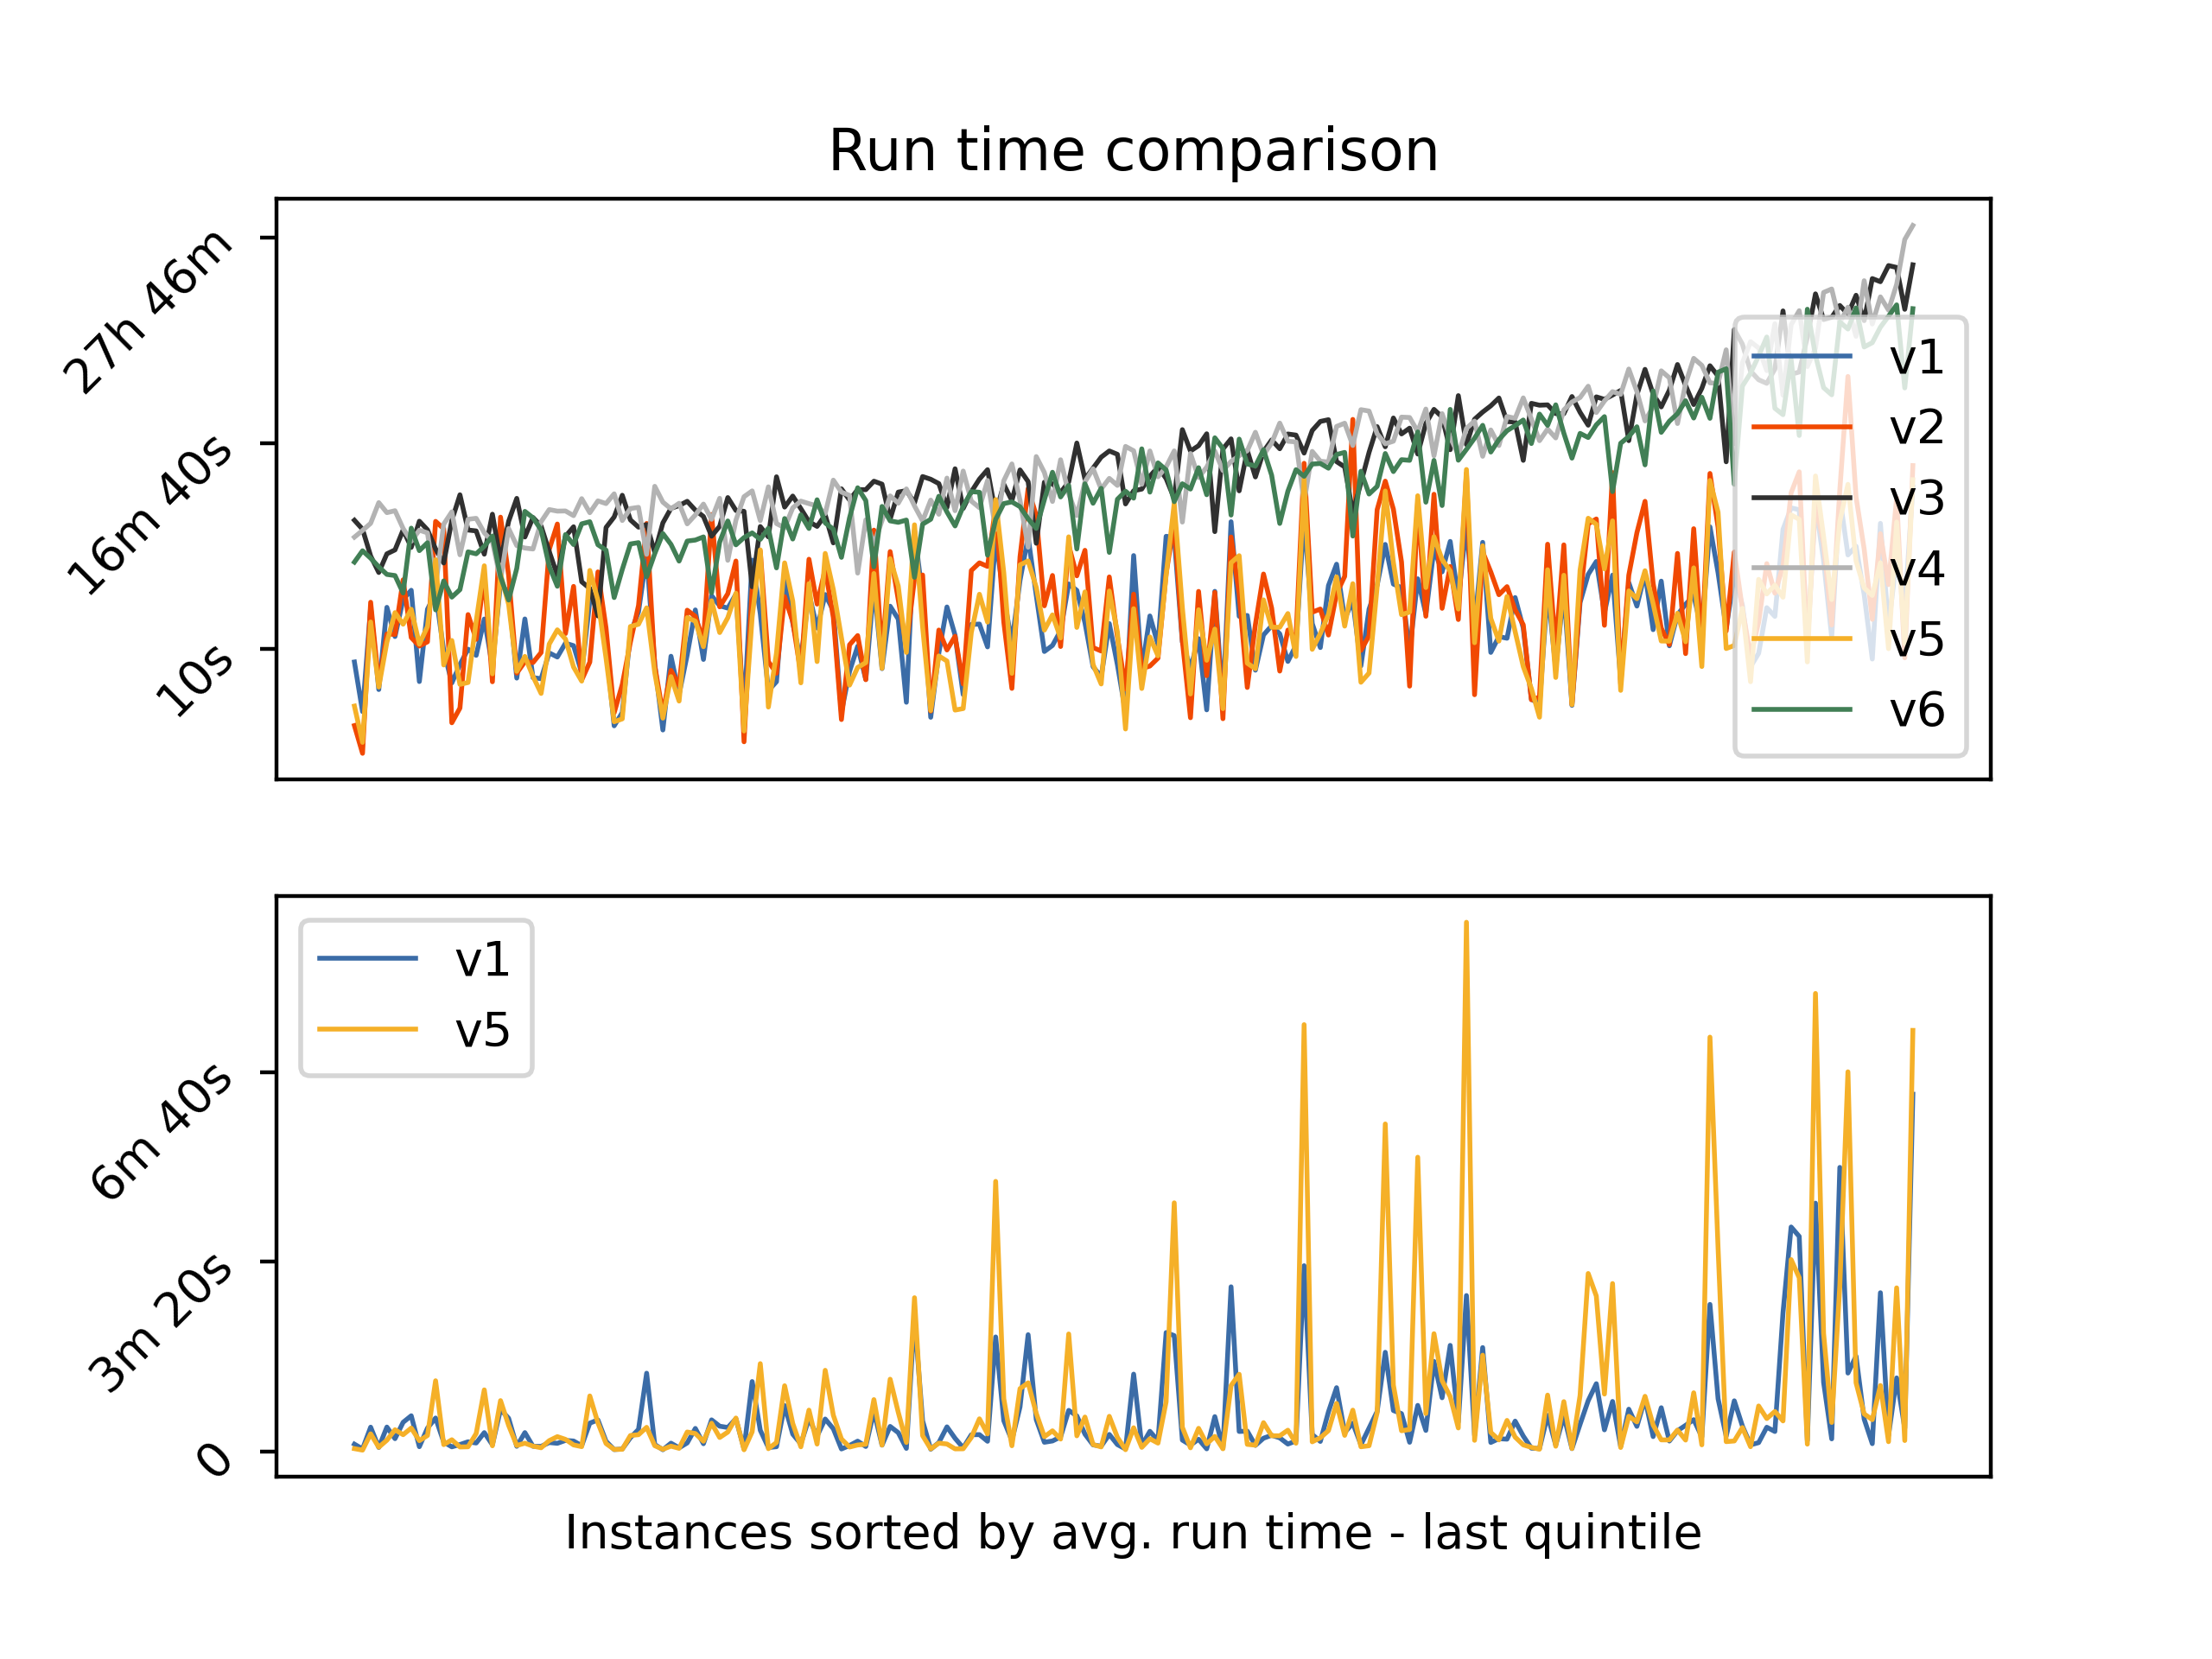
\includegraphics[width=12cm]{../resources/run_time_comparsion.png}
    \caption{Comparativa de el tiempo de ejecución de todas las versiones. Las instancias, en las abcisas, fueron ordenadas en orden creciente segun el tiempo promedio de ejecución de todas las versiones. En la primer gráfica la escala es logarítmica dado que los valores a comparar oscilan entre pocos segundos y casi treinta horas, en la segunda la escala es lineal. Se tomaron las últimas 200 instancias dado que eran las que presentaban diferencia más notoria.}
    \label{fig:runtimecomparison}
  \end{figure}

  \begin{figure}[h!]
    \centering
    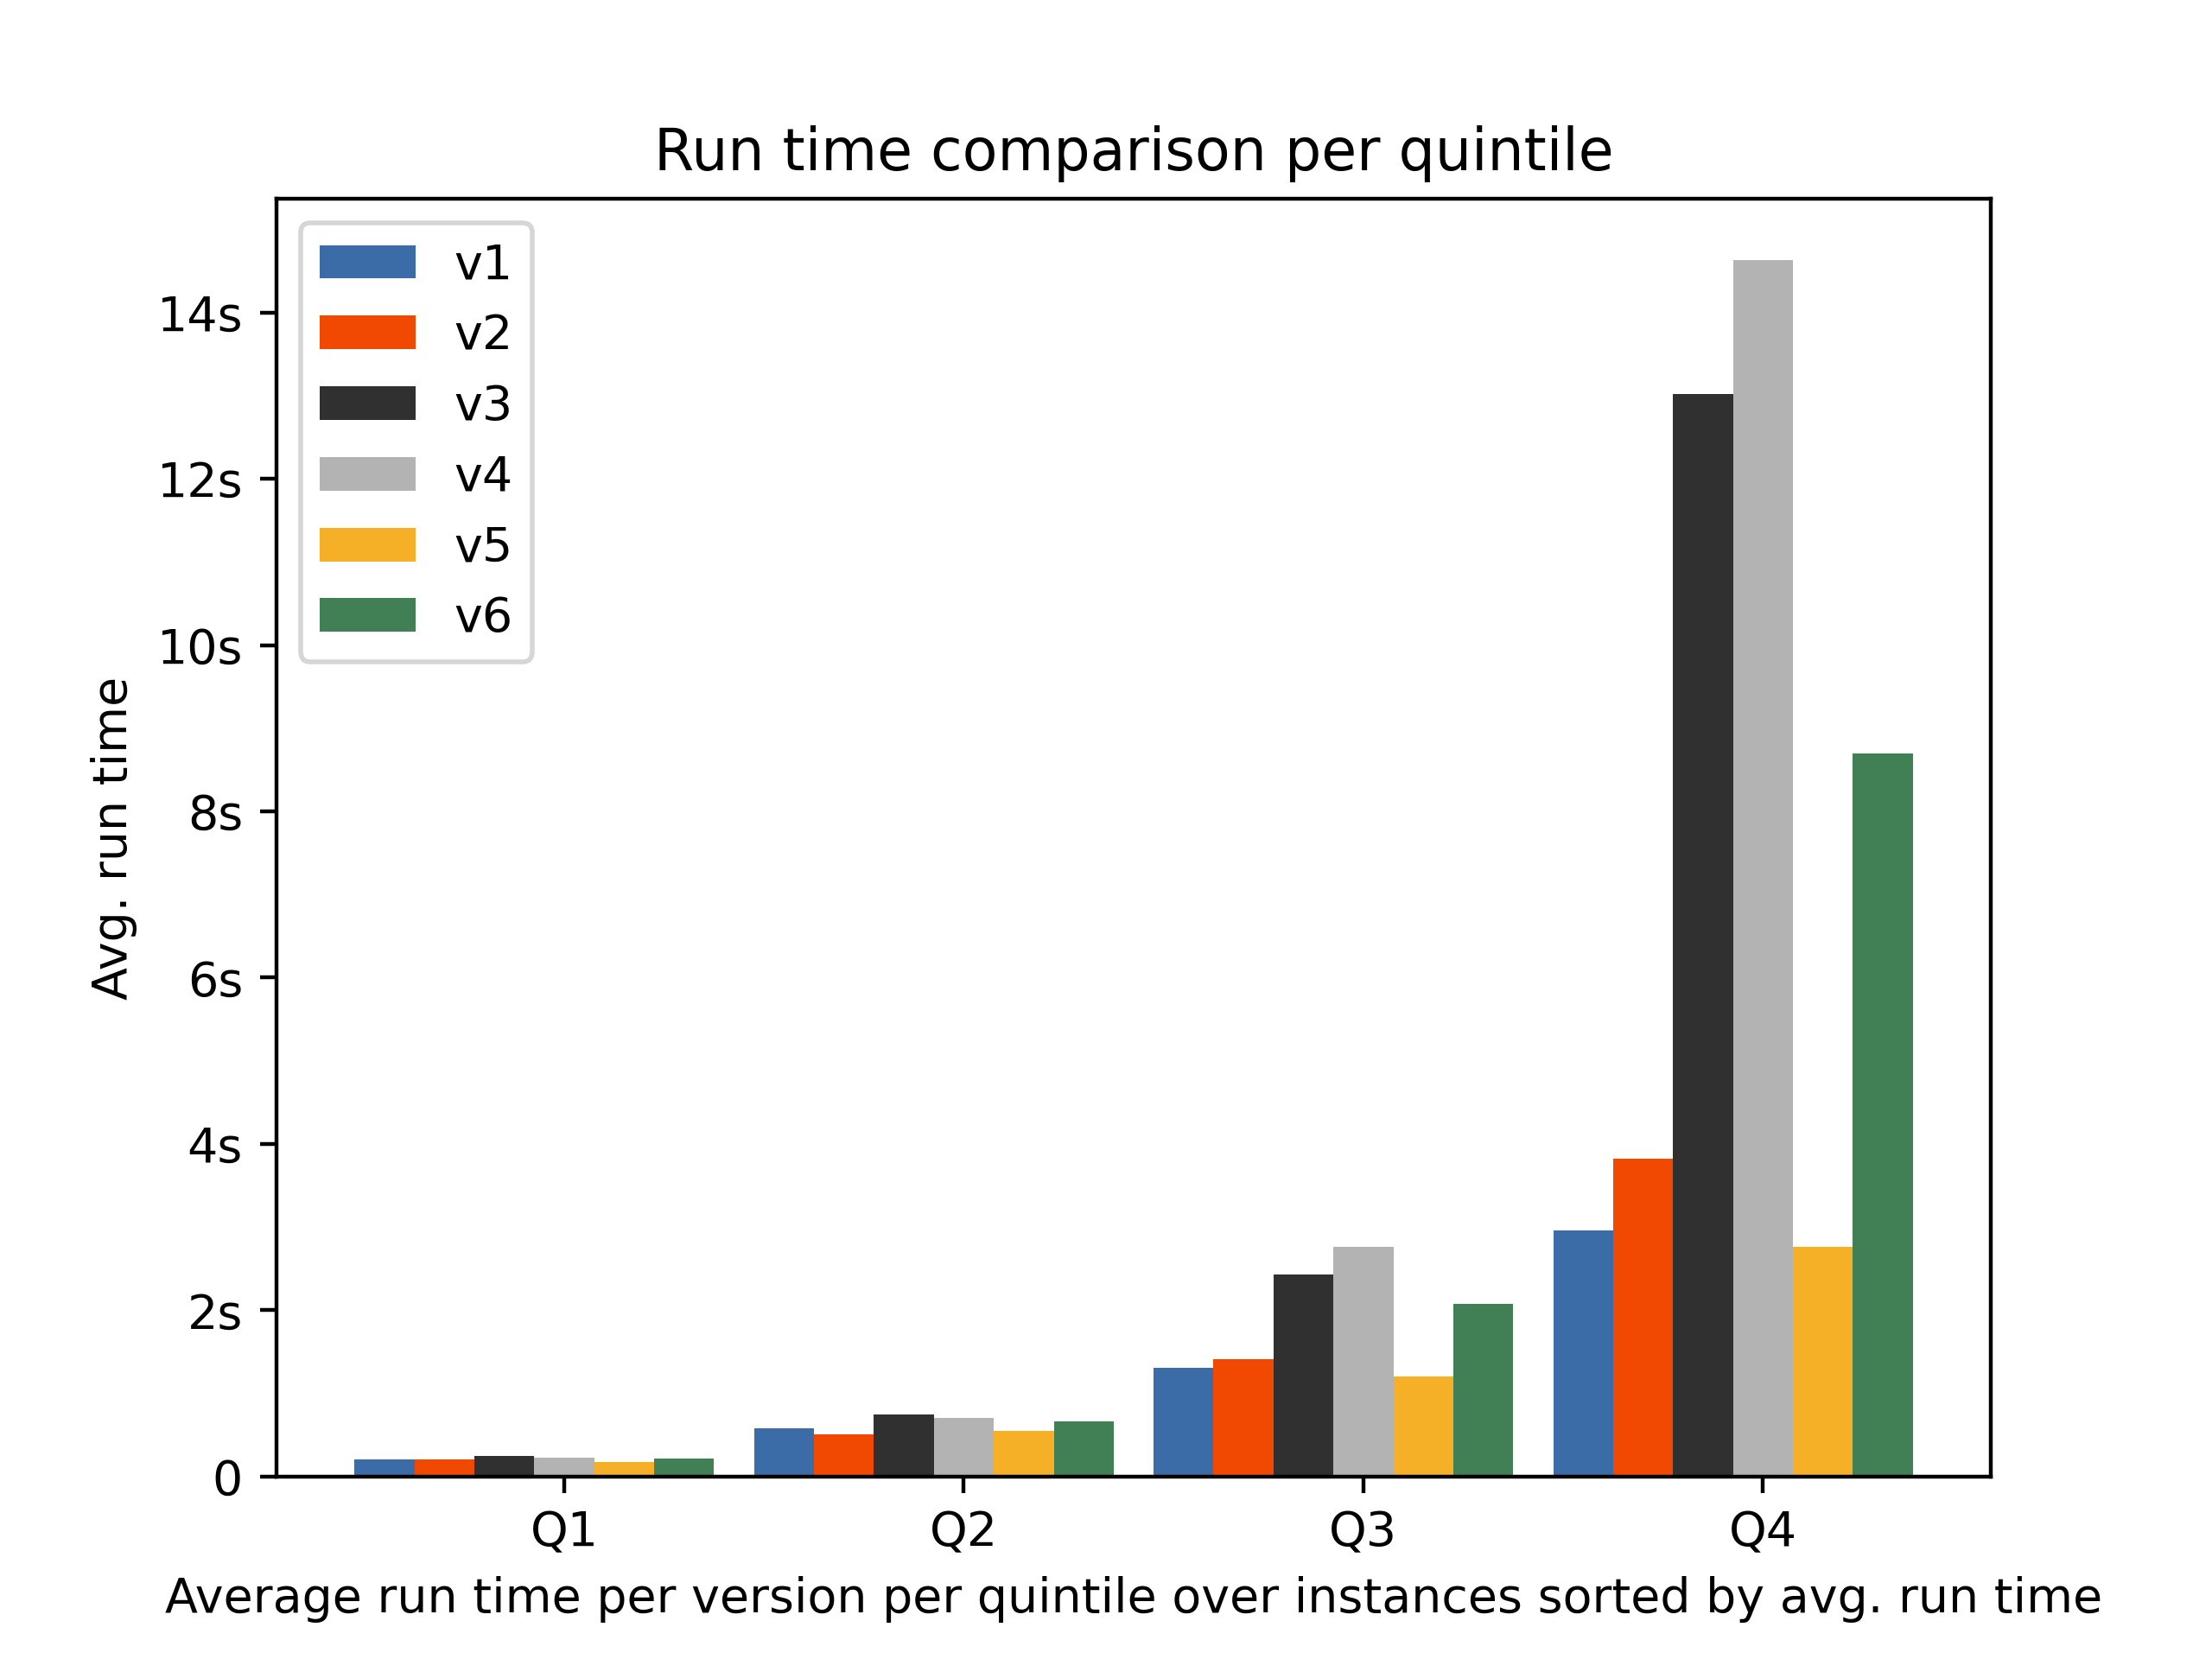
\includegraphics[width=12cm]{../resources/run_time_comparsion_by_quintile.png}
      \caption{Comparativa de el tiempo de ejecución de todas las versiones en tiempo promedio para los cuatro primeros quintiles. El promedio de las ejecuciones es en el tiempo promedio acumulado.}
    \label{fig:firstfourquintiles}
  \end{figure}

  El siguiente aspecto a tener en cuenta es el tiempo de ejecución. El tiempo de ejecución promedio nos da una medida gruesa para comparar y descartar algunas versiones. Las versiones v3, v4 y v6, que utilizan la formulación v1 de $f_k$ tienen un valor significativamente más alto que las otras, que utilizan la otra versión. Es de interés determinar si esta diferencia se da por algun tipo de instancia particular y si alguna versión se desempeña significativamente mejor en terminos de tiempo de ejecución si se quitan las posibles instancias dificiles. En la figura (\ref{fig:runtimecomparison}) se puede comparar el tiempo de ejecución de las versiones en las instancias mas dificiles de las generadas. Las versiones con mayor tiempo de ejecución promedio muestran una clara diferencia con las otras. Tambien se comparan las dos versiones con menor tiempo promedio de ejecución, donde se observa que la v1 es en la gran mayoría de los casos la más rápida. Para las instancias mas sencillas, primeros cuatro quintiles en figura (\ref{fig:firstfourquintiles}) los tiempos de ejecución no varían demasiado entre instancias y solo hacia el quintil cuatro se notan algunas diferencias aunque estas son de algunos segundos.

  Considerando el tiempo de ejecución promedio y el hecho de que no hubo incumplimientos en los chequeos se eligió la segunda version de formulación de $f_k$ con variables de holgura $r$, es decir la formulación v1, como formulación a utilizar en el resto de este trabajo.

  \subsection*{Especificación de datos}

  La formulación requiere la presencia de parámetros que en la práctica son de dificil o no son facilmente especificables en términos de un valor escalar. La cantidad y tipos de infrastructuras de ciclovía varían de país a país tanto en su disponibilidad como en sus costos, aún para el caso de Uruguay es dificil estimar, para las infrastructuras disponibles, sus costos de manera general ya que estos varían de la ubicación, congestión del área de la ciudad, precios de insumos como petroleo y mano de obra, reubicación de paradas de ómnibus y señales de tránsito, como se analiza en el analisis {\it Typical Costs of Cycling Interventions} (\ref{typicalcostsofcylcing}). Podemos simplificar los costos reportados en dicho análisis de manera de poder generalizarlos: decimos que la infrastructura de nivel $i+1$ cuesta el doble que la infrastructura de nivel $i$.

  Los costos de usuarios de atravesar un arco varían en la práctica de factores como ancho de la vía, pavimento, volumen y velocidad del tránstio, entre otros factores, a su vez ponderado por el largo del arco. En el documento {\it Bicycle Level Of Service, Applied Model} (\ref{blos2007}) podemos encontrar el concepto de {\it Bicycle Level of Service} (BLOS), muy utilizado en la literatura, que agrupa estas consideracionen bajo un único valor. Para el cálculo del BLOS se tienen en cuenta los siguientes aspectos, que cuantificados en indicadores luego son utilizados en una fórmula para calcular el puntaje de BLOS que por simplificación se estratifican en 6 niveles del A al F.

  \begin{enumerate}
    \item{Ancho promedio de la banquina, presencia de ciclovía, porcentaje de la vía ocupada por estacionamiento}
    \item{Límite de velocidad de vehículos motorizados}
    \item{Volumen promedio de los vehículos motorizados}
    \item{Porcentage de tránsito pesados (camiones)}
    \item{Condición del pavimento}
  \end{enumerate}

  \begin{table}[h!]
    \centering
    \caption*{{\bf Niveles de BLOS}}
    \begin{tabular}{cccc}
      \toprule
        Nivel & Puntaje BLOS & Infrastructura & Proporción del costo base \\
        A     & $\leq 1.5$   & 5              & 0.4   \\
        B     & 1.5-2.5      & 4              & 0.52  \\
        C     & 2.5-3.5      & 3              & 0.64  \\
        D     & 3.5-4.5      & 2              & 0.76  \\
        E     & 4.5-5.5      & 1              & 0.88  \\
        F     & > 5.5        & 0              & 1     \\
      \midrule
      \bottomrule
    \end{tabular}
    \caption{Niveles de servicio definidos en el BLOS, menor puntaje BLOS es mejor. Para cada nivel se define una infrastructura y su correspondiente proporción de mejora sobre la infrastructura base.}\label{table:blosscores}
  \end{table}

  Tomando como base el puntaje de BLOS estratificado, podemos traducir aproximadamente los puntajes a proporción de mejora de un nivel a otro utilizando la función $C_{infra}(i) = {(28 - 3 (i + 1)) \over 25}$, donde $i \in \{0,1,2,\ldots\}$ es la infrastructura, contrario a lo que define el estandar de BLOS, mientras mayor es el índice, mejor es la experiencia de usuario. Suponiendo que F corresponde a infrastructura base (o infrastructura 0), la proporción de mejora de las infrastructuras A-F correspondientes a las 1-5 se pueden observar en la tabla  (\ref{table:blosscores}).

  Para establecer una linea base sobre el comportamiento de las funciones de transferencia de demanda, que por simplicidad, asumimos que todas las $f_k$ se comportan igual. Es decir que $f_k(w_k) = f({w_k \over S^{best}_k})D_k$, donde $D_k$ es la demanda máxima que se puede transferir, $S^{best}_k$ es el costo del camino mas corto sobre la inrfastructura base y $f(x) \in [0, 1], x \in [0, 1]$ modela la proporción de demanda transferida en función de la proporción de $S^{best}_k$ lograda.

  Partimos del trabajo {\it Performance evaluation of extreme bicycle scenarios} (\ref{shwe2014}) que, analizando una extensiva encuesta realizada en varios países, aproxima a grosomodo una relación lineal entre la proporción de viajes hechos en bicicleta y el largo de infrastructura de ciclovía per cápita. Siguiendo este razonamiento asumiremos la $f$ baselineal decreciente, es decir que, a menor costo de usuario percibido se obtiene mayor atracción de demanda o mayor proporción de viajes en bicicleta. Se investigarán también algunas alternativas a $f$ como función logística inversa, logarítmica y exponencial.

  Establecer valores de presupuesto realistas depende altamente de de las condiciones políticas y económicas de cada localidad. Por simplicidad, especificaremos el presupuesto en función del costo total de la infrastructura de ciclovía inmediatamente mejor a la base construible. Podemos encontrar (TODO: donde?) que factores de presupuesto del 10\% a 40\% del total de la superficie estan dentro de los parámetros normales.

  Finalmente, usaremos la distancia de los arcos como costo de usuario y costo de la infrastructura base. Esto nos da una medida suficientemente simple y general como para usar en cualquier instancia y representativa.

  \subsection*{Análsis de sensibilidad}

  En esta sección se analiza cómo afectan las perturbaciones en los datos a las soluciones. Se utilizará la red de Sioux-Falls nuevamente dado que es de un tamaño manejable para realizar todas las ejecuciones en tiempo razonable. Se han dejado los datos de la red fijos y se estudiarán los parámetros especificos del problema, estos son: cantidad de infraestructuras, puntos de quiebre y presupuesto. La matriz de demanda se toma de Liu 2019 (\ref{liu2019}), con 22 pares origen-destino.

  En esta sección se busca determinar que características deben tener ciertos parámetros para que la formulaciones devuelva mejores resultados, mas allá de incrementos en el presupuesto. La cantidad de infraestructuras disponibles en una instancia es determinante respecto a la mejora de los caminos, es de esperar que la formulación decida utilizar mejores infraestructuras en los arcos con mayores flujo tanto como el presupuesto lo habilite y la demanda transferida lo amerite. En principio no hay sentido para limitar este número a un valor distinto al mayor posible a menos que el deteriorio en el tiempo de ejecución en comparación a los beneficios en terminos de demanda transferida sea inmanejable. Respecto a los puntos de quiebre se espera que una mayor granuladidad aporte positivamente al valor objetivo logrado aunque, de nuevo, se analizará el deterioro en el desempeño.

  Sobre el grafo y matriz de demanda antedichos, se agregan los siguientes parámetros base, que coinciden de la sección de especificación de datos:

  \begin{description}
    \item[Infrastructuras]: Se utilizan 5 infraestructuras ademas de la base.
    \item[Puntos de quiebre]: Consideramos la función lineal de transferencia de demanda con 5 puntos de quiebre.
    \item[Presupuesto]: Se establece un factor de presupuesto del 40\% .
  \end{description}

  \subsubsection*{Perturbaciones}

  Se analizaran las perturbaciones sobre el conjunto de parámetros base aplicando una perturbación de un parámetro por vez. Analizaremos alternar la cantidad de infrastructuras a las dos peores, ademas de la base. También se perturbará el factor de presupuesto entre valores de 10\%, 60\% y 80\%, con el objetivo de observar si se cumple la burda intuición de que siempre a mayor presupuesto se obtienen mejores resultados.

  Finalmente, se analizará en mayor profundidad la forma de especificar la función $f$ y los puntos de quiebre. En particular, se alternará entre 5 y 10 puntos de quiebre, se definirán los puntos de manera que sean equidistantes en el codominio de $f$, es decir que si hay N puntos, de un punto al siguiente se obtenga una mejora de $1/N$ en la proporción de demanda transferida. Se utilizarán las cuatro funciones de la figura (\ref{fig:fcatalog}).

  \begin{figure}[h!]
    \centering
    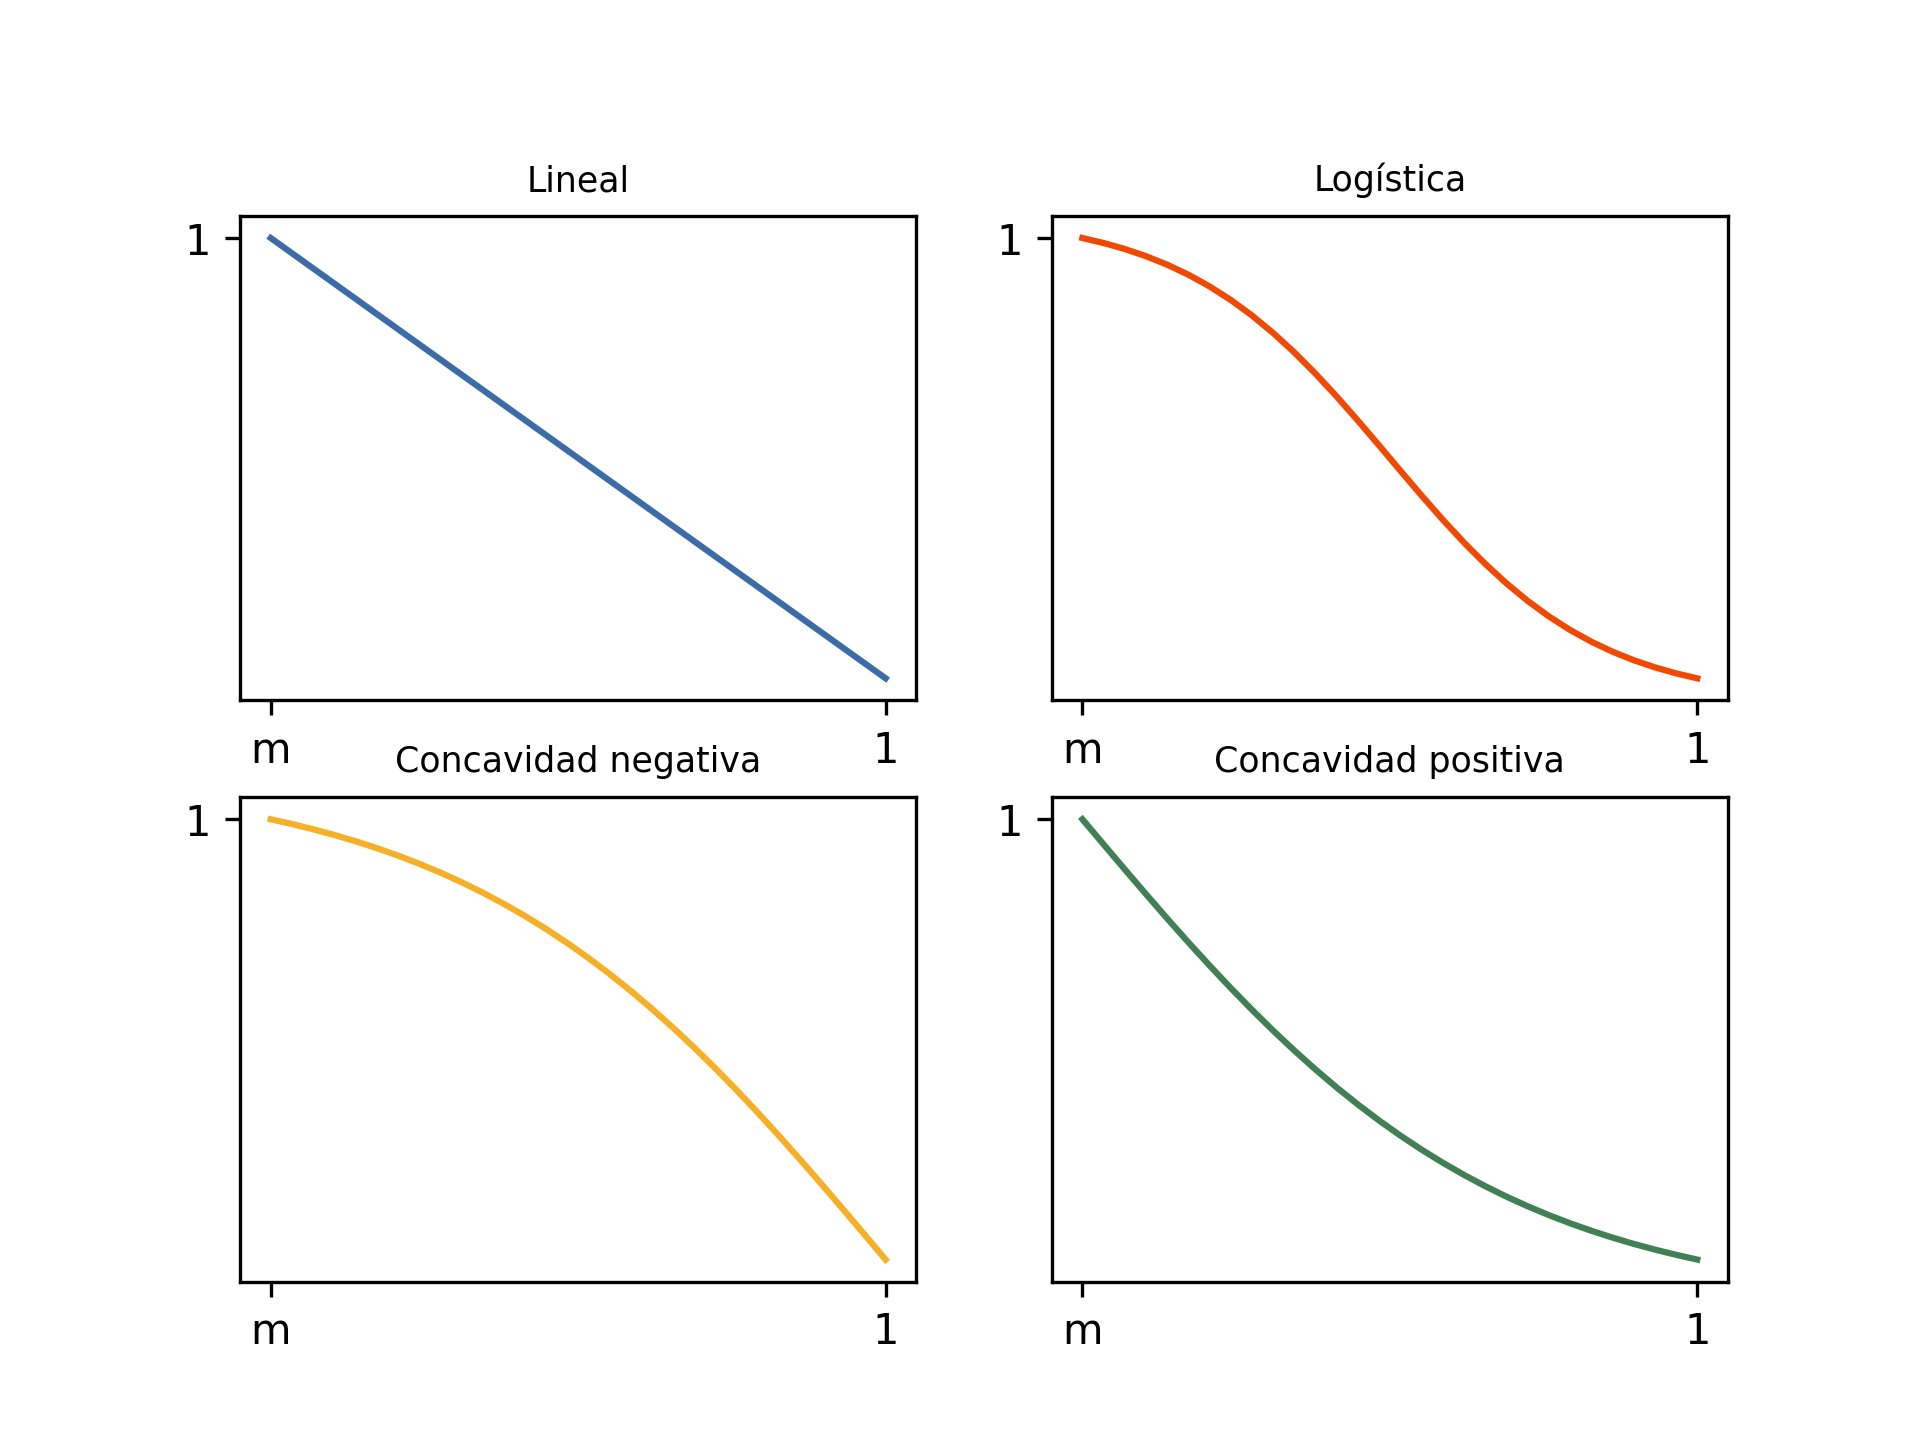
\includegraphics[width=8cm]{../resources/f_catalog.png}
      \caption{Catálogo de funciones $f$ usadas para modelar la transferencia de demanda a la bicicleta. El valor de $m$ varía segun las infrastructuras utilizadas y equivale a la proporción mínima alcanzada por la mejor infrastructura utilizada, es decir $m = min_{i \in I} \{ C_{infra}(i) \}$.}
    \label{fig:fcatalog}
  \end{figure}

  \section*{Resultados experimentales}

  Se probó la formulación final en la instancia de Montevideo de manera de poder analizar su aplicación práctica sobre datos familiares y poder compararlos con trabajos similares enmarcados dentro del proyecto CSIC "Diseño óptimo de redes de ciclovias".

  % TODO: Descripción de la instancia
  % - arcos, nodos, centroides
  % - matriz demanda: origen datos
  % - datos de demanda transferida: inventados seguramente

  \subsubsection*{Comparación frente a otros problemas}

  TODO: aca comparar los resultados con el otro problema de ciclovias trabajado como parte del proyecto de ciclovias.

  \section*{Detalles de implementación}

  Para facilitar la ejecución de instancias, se desarrollo una pequeña biblioteca que permite la especificación de una red y sus datos asociados de manera prográmatica para luego exportarla al tipo de datos que el modelo soportado por el solver.

  Las redes analizadas deben tener una serie de datos asociados de manera que sea posible solucionarlas con el modelo planteado. Para los nodos es necesario (no estrictamente) tener su par de coordenadas, para los arcos, se necesitan los siguientes atributos:

  \begin{description}
    \item[distance]: Distancia o longitud del arco.
    \item[user\_cost]: Costo de usuario de atravesar el arco sobre el grafo base (sin infraestructura o con la infraestructura base $i_0$).
    \item[construction\_cost]: Costo de construcción de la infraestructura base.
  \end{description}

  Luego, si se tienen $N$ infraestructura, para la infraestructura $n$ se calcula el costo de usuario de atravesarla como $user\_cost (-3 (n + 1) + 28) / 25$. El valor del costo de construcción será $2 n construction\_cost$. De ser necesario, pueden especificarse valores particulares de costos de dicha infraestructura para un arco mediante la utilización de los atributos $user\_cost\_n$ y $construction\_cost\_n$.

  \section*{Referencias}

  \begin{enumerate}
      \item{\label{heartrisksuy} MSP (2004). Investigación sobre factores de riesgo cardiovascular en Uruguay.}
    \item{\label{mspphisicalactivityguid} MSP. ¡A MOVERSE! Guia de actividad física.}
    \item{\label{mspsurveyriskfactors} MSP. Encuesta Nacional de Factores de Riesgo de Enfermedades no transmisibles.}
    \item{\label{bardbook} Jonathan F. Bard (1998). Practical Bilevel Optimization, Algorithms and Applications}
    \item{\label{laporte2007} Gilbert Laporte, Ángel Marín, et al. (2007). An Integrated Methodology for the Rapid Transit Network Design Problem}
    \item{\label{lim2021}} Jisoon Lim, Kevin Dalmeijer, et al. (2021). he Bicycle Network Improvement Problem:
    Optimization Algorithms and A Case Study in Atlanta.
    \item{\label{transportationnetworkrepo} Transportation Networks Repositort \url{https://github.com/bstabler/TransportationNetworks}}
    \item{\label{liu2019} Haoxiang Liu, Haoxiang Liu and Jiancheng Long (2019). Bike network design problem with a path-size logit-based equilibrium constraint: Formulation, global optimization and matheuristic.}
    \item{\label{typicalcostsofcylcing} UK Department for Transport (2017). Typical Costs of Cycling Interventions Interim analysis of Cycle City Ambition schemes.}
    \item{\label{blos2007} Sprinkle Consulting Inc. (2007), Bicycle Level Of Service, Applied Model.}
    \item{\label{shwe2014} Schweizer y Rupi (2014). Performance evaluation of extreme bicycle scenarios.}
  \end{enumerate}
\end{document}
